\section{Independent Test Results}
\begin{figure*}[t]
\centering
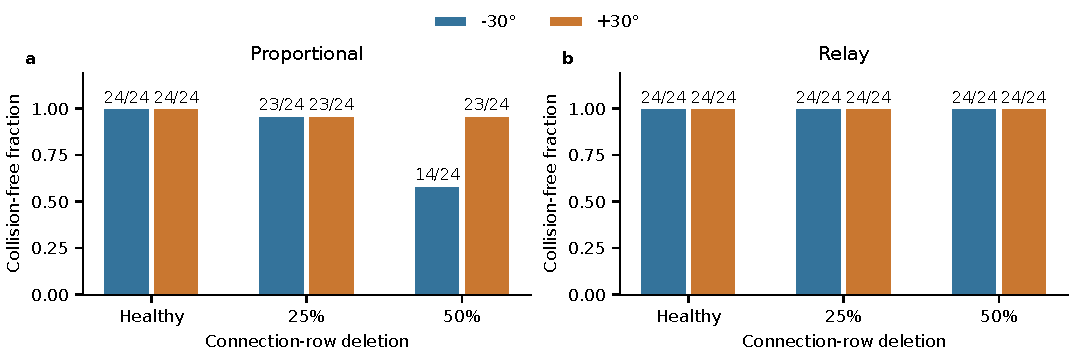
\includegraphics[width=\textwidth]{figs/task_v9_outcomes.pdf}
\caption{All independent core outcomes at the fixed 1-s task horizon. Each bar contains 24 seed clusters; the two directions, laws and doses within a seed are paired, not independent replicates. Counts are raw successes/episodes. Both healthy directions succeed under both laws; 50\% deletion produces different task loss despite the common mask and actuator limits.}
\label{fig:v9-outcomes}
\end{figure*}
\subsection{Fault Loss Depends on Feedback}
All 96 healthy core episodes succeed: 24/24 for each law/bearing in Fig.~\ref{fig:v9-outcomes}. At 25\% deletion, proportional control succeeds in 46/48 episodes and relay in 48/48; at 50\%, these counts are 37/48 and 48/48. There are no healthy-to-fault gains. The 50\% proportional losses are direction-dependent: 10/24 at $-30^\circ$, 1/24 at $+30^\circ$. Both healthy directions remain capable, avoiding the earlier directional floor.

The registered relay-minus-proportional net-loss contrast at 50\% is $-22.9$ percentage points (pp), 95\% cluster interval $[-33.3,-12.5]$, with 11/24 nonzero cluster contrasts. Symmetric-null sign-flip sensitivity gives raw $p=0.000977$, Holm-adjusted $p=0.00195$. At 25\%, the contrast is $-4.2$\,pp, interval $[-10.4,0]$, adjusted $p=0.50$; two nonzero clusters provide limited evidence. Relay's zero losses are observations, not zero-risk estimates. These new laws do not replicate the older six-cluster original/gated comparison, whose exploratory 25\% $p=0.25$ remains in the supplement.



A post-hoc trace diagnostic finds identical trigger times and pre-decision traces in all 144 matched law/scenario pairs. Steering is gated below the trigger threshold, so the laws first diverge after that decision. Median trigger time rises from 160 to 220\,ms under 50\% deletion for both laws; median absolute heading at the precontact 400-ms window is $38.7^\circ$ for proportional control and $96.0^\circ$ for relay. This describes a timing/turning pathway, not an identified mediation effect. Maximum turn rates match; executed turning effort does not. The result concerns feedback context rather than an intrinsically more fault-tolerant network.

\subsection{Neural Criteria Miss Task Failures}
All 400-ms assessments precede the earliest contact, 607.6\,ms. Table~\ref{tab:v9-warnings} scores the same 288 records against 13 later collisions and 275 successful tasks. The command-rate criterion detects only 2/13 collisions; its sensitivity interval is $[0,40.0]\%$. Two-sided activity detects 3/13 with more false alarms, and the upper activity limit detects none. Thus, simply adding a lower activity cutoff does not resolve the endpoint mismatch.

\begin{table}[t]
\caption{Frozen 400-ms warnings on all core records. TP/FN use 13 collisions; FP uses 275 successful tasks. Full cluster intervals, specificity, FPR and FNR are in the supplement. These are scores of our records, not executions of SpikeFI or SpikingJET.}
\label{tab:v9-warnings}
\centering
\begin{tabular}{lrrrrr}
\toprule
Criterion & TP & FP & FN & Sens. (\%) & FPR (\%)\\
\midrule
Command low & 2 & 51 & 11 & 15.4 & 18.5\\
Activity upper & 0 & 0 & 13 & 0.0 & 0.0\\
Activity two-sided & 3 & 68 & 10 & 23.1 & 24.7\\
Actuator schedule & 13 & 84 & 0 & 100.0 & 30.5\\
Held command & 13 & 57 & 0 & 100.0 & 20.7\\
\bottomrule
\end{tabular}
\end{table}

Both geometry-informed forecasts detect 13/13 collisions. Holding the current neural turn command reduces false alarms from 84 to 57 relative to the same-state zero-future-turn baseline. A secondary descriptive paired analysis gives a specificity gain of 9.8\,pp, interval $[6.6,13.4]$. Its remaining 20.7\% false-alarm rate and exact-state information limit practical interpretation. Zero observed misses yield a degenerate bootstrap interval; the one-sided 95\% bound on any miss in a new, identically defined seed cluster is 11.7\%, not a conditional FNR guarantee. This candidate is not a validated protection algorithm.

\subsection{Horizon and Exposure Have Distinct Effects}
Only two collisions occur by 800 or 900\,ms, versus 13 by 1\,s. The 50\% controller contrast is therefore $-4.2$\,pp at the earlier horizons, versus $-22.9$\,pp at 1\,s. These are repeated observations, not extra samples; the declared horizon materially changes task loss.

In contrast, duration matching leaves every group median spike ratio unchanged. At 50\% deletion, stopped/common medians are 1.505 for proportional control and 1.257 for relay; the maximum individual change over all pairs is 0.00325. The large historical stopped/common difference does not recur here. Proportional 50\% activity has median ratio 0.981 at 400\,ms and 1.505 over 1\,s, illustrating distinct resource windows. Full-horizon post-contact continuation is not prospective warning evidence.
